% ==========================
\chapter{Recovery by Repair}
\label{chap:repair}
% ==========================

The unprotected limit study showed that instruction memory fails deterministically once faults persist in static storage. 
Resets and detection mechanisms provide no recovery because corrupted instructions are re-executed identically after every reboot. 
This behavior defines the lower bound of software reliability—where faults in code itself permanently prevent progress.  

To move beyond detection, the system must regenerate correct behavior from within the same faulty memory space. 
\textbf{Repair} achieves this by algorithmically reconstructing code or data from redundant or overlapping information, 
producing a more reliable version of the original content. 
Unlike reset-based recovery, repair operates in place, fusing imperfect data to restore an executable state.  

This chapter introduces repair as the first active recovery mechanism for static memory faults. 
It evaluates two representative models—\textbf{Majority-of-3} and \textbf{Reed–Solomon (255,223)}—that combine information from multiple unreliable regions to reconstruct usable code. 
Both approaches operate entirely within memory, without reboot or external reprogramming, and aim to restore a coherent instruction stream by reinforcing correct content through redundancy.  

% ---------------------------------------------------
\section{Overview}
\label{sec:repair-overview}
% ---------------------------------------------------

The following sections develop a quantitative model of repair, derive analytical expressions for survivability, 
and validate these models through a limit study that measures how repair strength and redundancy influence system reliability. 
These results establish repair as a baseline mechanism for sustaining execution when persistent instruction corruption 
would otherwise render the system non-recoverable.

\section{Repair Survivability}
\label{sec:repair-survivability}

Repair mechanisms improve system survivability by introducing structured redundancy into static memory.  
They increase the likelihood that usable code or data can be reconstructed directly from within the same faulty region.  
Each protected area contains two main components: a \textit{source block} that holds the original content and one or more \textit{redundant blocks} that encode overlapping or supplementary information derived from it.  
When corruption occurs, these blocks are combined algorithmically to form a reconstructed version that has a higher probability of being correct than any individual block alone.

Two representative forms of repair are considered: \textbf{Majority-of-3} replication and the \textbf{Reed--Solomon (255,223)} code.  
Both rely on redundancy but differ in structure, efficiency, and computational cost.  

\subsection{Majority-of-3}

Majority-of-3 is a replication-based approach in which three identical copies of each bit are stored.  
During repair, the most common value among the three is selected, allowing a correct bit to be recovered as long as two of the three replicas remain uncorrupted.  
This scheme is simple and effective against isolated bit errors but requires significant storage overhead—two-thirds of all stored bits are redundant.

Let $p_f$ denote the probability that a single bit is faulty.  
For any given bit position, let $X \sim \mathrm{Binomial}(3, 1 - p_f)$ represent the number of fault-free replicas.  
The fused bit is fault-free if $X \ge 2$, giving the per-bit survivability:

\begin{equation}
P_{\text{bit,maj3}} = \sum_{k=2}^{3} \binom{3}{k} (1 - p_f)^k p_f^{3-k} = 1 - 3p_f^2 + 2p_f^3.
\end{equation}

If $S$ bytes of memory are protected by Majority-of-3, the total number of fused bits is $\tfrac{8S}{3}$, yielding whole-memory survivability:

\begin{equation}
p_{\text{free,maj3}}(S, p_f) = (1 - 3p_f^2 + 2p_f^3)^{\tfrac{8S}{3}}.
\end{equation}

This model captures how redundancy statistically suppresses bit-level faults but with a steep storage penalty.

\subsection{Reed--Solomon (RS(255,223))}

Reed--Solomon repair uses an algebraic method that distributes data and parity across groups of bytes.  
When a subset of these bytes becomes corrupted, missing or invalid data can be regenerated mathematically using the remaining bytes, provided the number of errors does not exceed the correction capacity of the code.  
The RS(255,223) configuration stores 223 data bytes and 32 parity bytes per codeword, achieving approximately 87\% efficiency and tolerating up to 16 corrupted bytes per block.

Let $p_f$ again denote the per-bit fault probability, and define the per-byte fault probability as:

\begin{equation}
q = 1 - (1 - p_f)^8.
\end{equation}

The probability that an RS(255,223) codeword is decodable—that is, that it contains at most 16 faulty bytes—is:

\begin{equation}
p_{\text{block,RS}}(q) = \sum_{j=0}^{16} \binom{255}{j} q^j (1 - q)^{255-j}.
\end{equation}

For a protected memory of size $S$ bytes, the number of full codewords is:

\begin{equation}
N_{\text{RS}} = \left\lceil \frac{S}{255} \right\rceil,
\end{equation}

and the total memory survivability is:

\begin{equation}
p_{\text{free,RS}}(S, p_f) = \left( p_{\text{block,RS}}(q) \right)^{N_{\text{RS}}}.
\end{equation}

This form shows how Reed--Solomon maintains high survivability until its correction threshold is exceeded, after which reliability collapses sharply.

\begin{figure}[t]
  \centering
  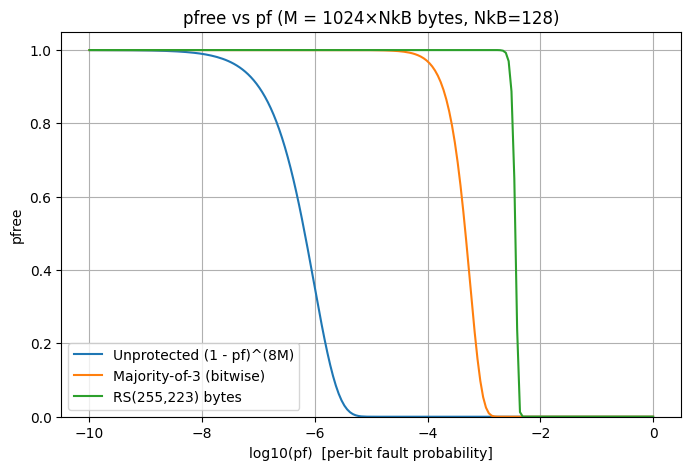
\includegraphics[width=\linewidth]{Chapter-4/figs/pfree-reed_maj.png}
  \caption{Modeled survivability of Majority-of-3 and Reed--Solomon (255,223) repair for a 128~kB memory region.  
  Each curve shows the probability of complete fault-free recovery as a function of per-bit fault probability $p_f$.  
  Both methods combine information from multiple unreliable \textit{source blocks} and their associated \textit{redundant blocks} to reconstruct usable data.  
  Majority-of-3 degrades gradually with fault density, while Reed--Solomon maintains near-perfect reliability until its decoding capacity is exceeded.}
  \label{fig:pfree-vs-pf-128kb}
\end{figure}

\subsection{Comparison and Interpretation}

Figure~\ref{fig:pfree-vs-pf-128kb} compares survivability for the two repair schemes over a 128~kB memory region.  
Both extend reliability several orders of magnitude beyond the unprotected baseline, but their behavior diverges under increasing corruption.  
Majority-of-3 exhibits a smooth, probabilistic decline as more replicas fail, while Reed--Solomon maintains a sharp threshold—perfect recovery below its correction limit and sudden collapse beyond it.  
This contrast illustrates the design trade-off between simplicity and efficiency: replication offers continuous but costly improvement, whereas coding provides near-ideal protection up to a fixed limit.  

These analytical results form the upper bound of repair performance.  
The following section empirically validates these models through controlled fault injection, measuring how closely practical repair aligns with the theoretical predictions.

\section{Limit Study}
\label{sec:ch3-limit-study}

The repair limit study quantifies how practical repair mechanisms behave when faults are directly injected into memory.  
While the analytical model predicts ideal survivability under the assumption of independent faults and perfect correction, 
this experiment measures how these theoretical benefits hold under real program conditions.  
It represents the transition from mathematical reliability to empirical system behavior.

In this study, both \textbf{Majority-of-3} and \textbf{Reed--Solomon (RS 255,223)} repair schemes are evaluated using 
the same probabilistic fault model introduced earlier.  
The per-bit fault probability is fixed at its maximum ($p_f = 1$), representing a fully fault-saturated environment.  
Rather than varying $p_f$ directly, the experiment varies the \textbf{injection rate} $R$, which defines the average 
spacing between corrupted bytes.  
Smaller $R$ values correspond to denser corruption, while larger $R$ values represent sparser, more isolated faults.  
This approach allows each repair mechanism’s reliability limit to be observed under progressively worsening fault density.

Each repair mechanism operates on a set of encoded binary images derived from the benchmark programs.  
The experimental workflow consists of four phases:

\begin{enumerate}
  \item \textbf{Encoding} – Each benchmark is transformed into a protected format using either Majority-of-3 replication 
  or Reed--Solomon coding.  
  The encoder generates redundant structures representing \textit{source} and \textit{redundant} blocks.

  \item \textbf{Fault Injection} – Corruption is applied to these encoded images following the Poisson--Uniform model.  
  Only the encoded memory is corrupted; decoder executables remain fault-free to isolate the effects of repair.

  \item \textbf{Decoding (Repair)} – Each corrupted image is decoded using its corresponding algorithm.  
  Majority-of-3 performs bitwise voting across replicas, while Reed--Solomon reconstructs codewords algebraically.

  \item \textbf{Validation} – The repaired outputs are executed and compared against known-good results.  
  Successful runs indicate complete and correct reconstruction, while mismatches or crashes indicate repair failure.
\end{enumerate}

\begin{figure}[t]
  \centering
  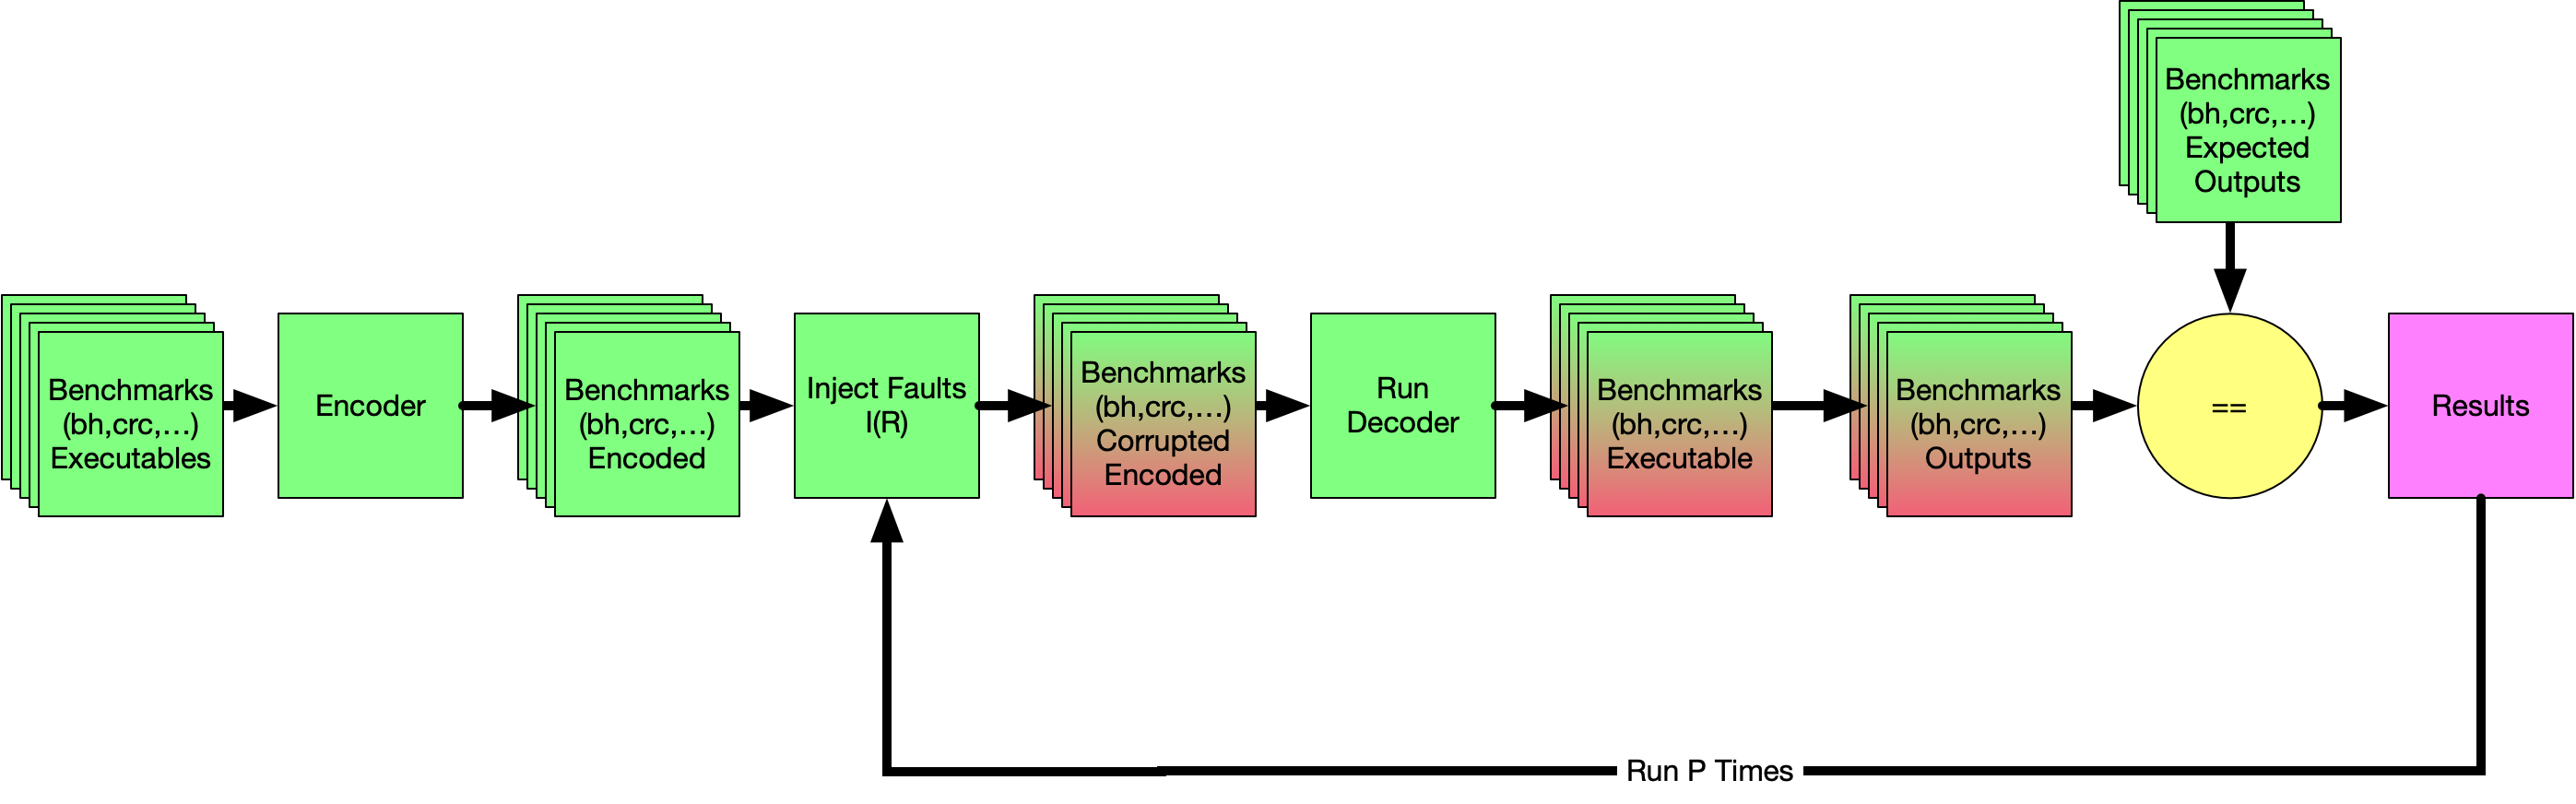
\includegraphics[width=\linewidth]{Chapter-4/figs/repair-flow.png}
  \caption{Repair limit-study workflow. Benchmarks are first \emph{encoded} (producing source and redundant blocks), then faults are \emph{injected} into the encoded images according to the Poisson--Uniform model. The corrupted images are \emph{decoded (repaired)}, yielding executable binaries that are run to produce outputs. Outputs are compared to known-good references; equality counts as success. The entire process is repeated \(P\) times per injection rate \(R\) to obtain empirical survivability.}
  \label{fig:repair-flow}
\end{figure}

The process is repeated multiple times for each injection rate $R$ to capture statistical variation.  
For each configuration, the fraction of successful reconstructions represents the measured system survivability.

\begin{figure}[t]
  \centering
  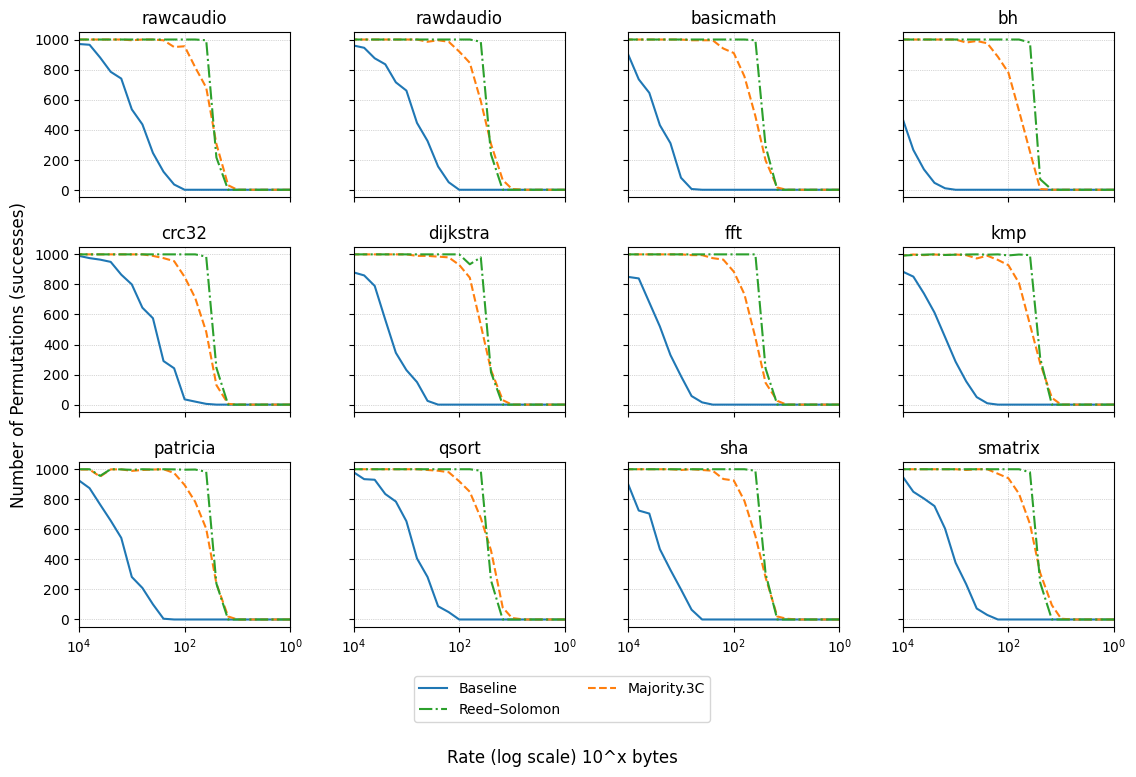
\includegraphics[width=\linewidth]{Chapter-4/figs/repair-reliability.png}
  \caption{Repair limit study results across benchmarks: number of successful permutations (out of $P$) versus injection rate $R$ (log scale).  
  Curves shown for Majority-of-3 and Reed--Solomon repair.  
  Both methods significantly extend functional survivability relative to the unprotected baseline.}
  \label{fig:repair-limit-results}
\end{figure}

\subsection{Results and Interpretation}
\label{subsec:ch3-limit-results}

The results show two distinct reliability profiles.  
\textbf{Majority-of-3} repair degrades gradually as the injection rate increases.  
Even under dense corruption, a fraction of systems continue to operate correctly because the probability of majority agreement remains nonzero.  
This produces a smooth, continuous decline in survivability, consistent with the probabilistic fusion of multiple noisy replicas.

\textbf{Reed--Solomon}, by contrast, exhibits a sharp threshold.  
For injection rates below its correction capacity, it achieves near-perfect reconstruction; once the number of corrupted bytes 
exceeds the 16-byte correction limit per codeword, reliability collapses almost instantaneously.  
This behavior matches the analytical model’s prediction: Reed--Solomon acts as a high-efficiency, high-risk boundary—
exceptionally effective within its limit but brittle beyond it.

Compared to the unprotected baseline, both methods extend survivability by several orders of magnitude.  
Reed--Solomon maintains integrity deeper into fault density, while Majority-of-3 offers graceful degradation rather than abrupt failure.  
Together, these results demonstrate the fundamental trade-off between replication and algebraic repair:  
replication consumes more memory to achieve continuity, while coding achieves higher efficiency at the cost of a strict correction boundary.

The repair limit study confirms that real-world repair follows the theoretical trends established in the analytical model.  
It also defines the practical boundaries of survivability—how redundancy interacts with fault density, how correction capacity scales, 
and where the probability of successful reconstruction drops below viability.  
These insights provide the foundation for applying repair in embedded systems, 
where memory access restrictions and runtime constraints further determine the feasibility of in-place recovery.

% ---------------------------------------------------
\section*{Repair Boundaries and the Need for Redirection}
% ---------------------------------------------------

While repair demonstrates that faulty code can sometimes be reconstructed from within the same memory space, 
its success depends on both the availability and integrity of writable regions. 
Even when a device supports in-system writes, the underlying memory cells may no longer accept updates once degraded—%
faults can permanently prevent the intended write or erase operation from succeeding. 
When this occurs, repair becomes ineffective because the correction cannot be physically applied.  
In these situations, reliability must come from structural redundancy rather than regeneration.  
The next chapter introduces \textbf{redirection by code replication}, in which multiple validated copies of code are pre-placed in memory, 
and execution dynamically shifts among them when corruption is detected.  
This approach extends survivability beyond the limits of repair by rerouting control flow through verified instruction paths 
instead of attempting to rewrite damaged storage.